% template copied from the 2017 new notes

\documentclass[a4paper,10pt]{article}
\usepackage[margin=0.5in]{geometry}
\usepackage{graphicx,color}
\usepackage{fullpage}
\usepackage{amsmath}
\usepackage{natbib}
\usepackage{amssymb}
\usepackage{bm}
\usepackage{ulem}
\usepackage{enumerate}
%\usepackage{aastex}

%\defcitealias{Chamandy+13a}{CSS13a}
%\defcitealias{Chamandy+13b}{CSS13b}
%\defcitealias{Comparetta+Quillen12}{CQ12}

\def\apj{ApJ}
\def\apss{Ap{\&}SS}
\def\mnras{MNRAS}
\def\aap{A\&A}
\def\apjl{ApJ}
\def\gafd{Geophys.\ Astrophys.\ Fluid Dyn.}
\def\jfm{JFM}
\def\physrep{PhR}
\def\pre{PRE}
\def\prl{PRL}
\def\apjs{ApJS}
\def\pasa{PASA}
\def\pasj{PASJ}
\def\nat{Natur}
\def\pasp{PASP}
\def\ssr{SSRv}
\def\araa{ARA\&A}
\def\aj{AJ}

\renewcommand{\vec}[1]{{{\mbox{\boldmath $#1$}}}}%also makes bold Greek letters
\newcommand{\ar}{_\mathrm{a}}
\newcommand{\aar}{\mathrm{,a}}
\newcommand{\ir}{_\mathrm{i}}
\newcommand{\iir}{\mathrm{,i}}


\newcommand{\sign}[1]{\textrm{sign}({#1})}
\newcommand{\zhat}{\hat{z}}
\newcommand{\bfzhat}{\bm{\hat{z}}}
\newcommand{\What}{\widehat{W}}
\newcommand{\Vhat}{\widehat{V}}
\newcommand{\Exp}[1]{{\rm e}^{#1}}
\newcommand{\Log}{\mathrm{Log}}
\newcommand{\del}{\partial}
\newcommand{\Del}{{\nabla}}
\newcommand{\bfDel}{\bm{\nabla}}
\newcommand{\bmDel}{\bm{\nabla}}
\newcommand{\bfomega}{\vec{\omega}}
\newcommand{\bmomega}{\vec{\omega}}
\newcommand{\bfOmega}{\vec{\Omega}}
\newcommand{\bmOmega}{\vec{\Omega}}
\newcommand{\bfgamma}{\vec{\gamma}}
\newcommand{\bmgamma}{\vec{\gamma}}
\newcommand{\alp}{\alpha}
\newcommand{\Gam}{\Gamma}
\newcommand{\eps}{\epsilon}
\newcommand{\Delsq}{\nabla^2}
\newcommand{\Emf}{\bm{\mathcal{E}}}
\newcommand{\Fmf}{\bm{F}}
\newcommand{\Flux}{\bm{\mathcal{F}}}
\newcommand{\flux}{\mathcal{F}}
\newcommand{\Bs}{\mathcal{B}}
\newcommand{\Bsr}{\mathcal{B}_r}
\newcommand{\Bsp}{\mathcal{B}_\phi}
\newcommand{\Bsz}{\mathcal{B}_z}
\newcommand{\bfU}{\bm{U}}
\newcommand{\bfB}{\bm{B}}
\newcommand{\bfJ}{\bm{J}}
\newcommand{\bfu}{\bm{u}}
\newcommand{\bfb}{\bm{b}}
\newcommand{\bmb}{\bm{b}}
\newcommand{\bfj}{\bm{j}}
\newcommand{\bmj}{\bm{j}}
\newcommand{\bfr}{\bm{r}}
\newcommand{\bfp}{\bm{\phi}}
\newcommand{\bfz}{\bm{z}}
\newcommand{\Emfr}{\mathcal{E}_r}
\newcommand{\Emfp}{\mathcal{E}_\phi}
\newcommand{\Emfz}{\mathcal{E}_z}
\newcommand{\Emfi}{\mathcal{E}_i}
\newcommand{\Fmfr}{F_r}
\newcommand{\Fmfp}{F_\phi}
\newcommand{\Fmfz}{F_z}
\newcommand{\Fluxr}{\mathcal{F}_r}
\newcommand{\Fluxphi}{\mathcal{F}_\phi}
\newcommand{\Fluxz}{\mathcal{F}_z}
\newcommand{\mean}[1]{\overline{#1}}
%\newcommand{\meanv}[1]{\overline{\bm{#1}}}
\newcommand{\meanv}[1]{\bm{#1}}
\newcommand{\avg}[1]{\left<{#1}\right>}
\newcommand{\corr}{_\mathrm{c}}						%correlation
\newcommand{\corot}{_\mathrm{c}}						%corotation
\newcommand{\D}{_\mathrm{D}}						%disc
\newcommand{\eq}{_\mathrm{eq}}						%equipartition
\newcommand{\eqdisk}{_\mathrm{eq,d}}						%equipartition
\newcommand{\eqhalo}{_\mathrm{eq,h}}						%equipartition
\newcommand{\rms}{_\mathrm{0}}						%rms
\newcommand{\f}{_\mathrm{0}}					   	%forcing
\newcommand{\forc}{_\mathrm{f}}					   	%forcing
\newcommand{\fdisk}{_\mathrm{0,d}}					   	%forcing
\newcommand{\fhalo}{_\mathrm{0,h}}					   	%forcing
\newcommand{\z}{_\mathrm{0}}					   	%forcing
\newcommand{\1}{_\mathrm{1}}					   	%forcing
\newcommand{\2}{_\mathrm{2}}					   	%forcing
\newcommand{\kin}{_\mathrm{k}}			   		%kinematic
\newcommand{\magn}{_\mathrm{m}}			   		%magnetic
\newcommand{\turb}{_\mathrm{t}}			   		%turbulent
\newcommand{\etat}{\eta_\mathrm{t}}			   	%turbulent diffusivity
\newcommand{\kappat}{\kappa_\mathrm{t}}			   	%turbulent diffusivity
\newcommand{\Turb}{\mathrm{t}}			   		%turbulent, in-line
\newcommand{\crit}{_\mathrm{c}}			   		%critical
\newcommand{\sat}{_\mathrm{sat}}			   		%critical
\newcommand{\magnsat}{_\mathrm{m,sat}}			   		%critical
\newcommand{\const}{\mathrm{const}}			   	%constant
\newcommand{\mx}{\mathrm{max}}			   		%maximum
\newcommand{\ma}{_\mathrm{max}}			   		%maximum
\newcommand{\dd}{\mathrm{d}}			   		%differential
\newcommand{\adv}{_\mathrm{a}}			   		%advection, subscript
\newcommand{\diff}{_\mathrm{d}}			   		%diffusion, subscript
\newcommand{\udiff}{^\mathrm{d}}			   		%diffusion, subscript
\newcommand{\pol}{_\mathrm{p}}			   		%poloidal, subscript
\newcommand{\diffzero}{_\mathrm{d,0}}
\newcommand{\num}{_\mathrm{num}}			   	%diffusion, subscript
\newcommand{\Adv}{\mathrm{a}}			   		%advection, subscript
\newcommand{\Diff}{\mathrm{d}}			   		%diffusion, in-line
\newcommand{\VC}{_\mathrm{VC}}			   		%diffusion, in-line
\newcommand{\uVC}{^\mathrm{VC}}			   		%diffusion, in-line
\newcommand{\on}{_0}
\newcommand{\off}{_\mathrm{off}}
\newcommand{\cro}{\times}
\newcommand{\Rm}{\mathcal{R}_\mathrm{m}}
\newcommand{\Rey}{\mathcal{R}_\mathrm{e}}
\newcommand{\mbr}{B_r}
\newcommand{\mbp}{B_\phi}
\newcommand{\mbz}{B_z}
\newcommand{\mbi}{B_i}
\newcommand{\mur}{U_r}
\newcommand{\mup}{U_\phi}
\newcommand{\muz}{U_z}
\newcommand{\muP}{U_\mathrm{p}}
\newcommand{\muztilde}{\widetilde{\mean{U}}_z}
\newcommand{\mui}{\mean{U}_i}
\newcommand{\tautilde}{\widetilde{\tau}}
\newcommand{\gammatilde}{\widetilde{\gamma}}
\newcommand{\alphatilde}{\widetilde{\alpha}}
\newcommand{\kappatilde}{\widetilde{\kappa}}
\newcommand{\alptilde}{\alphatilde}
\newcommand{\omegatilde}{\widetilde{\omega}}
\newcommand{\omtilde}{\omegatilde}
\newcommand{\Ctilde}{\widetilde{C}}
\newcommand{\rtilde}{\widetilde{r}}
\newcommand{\qtilde}{\widetilde{q}}
\newcommand{\atilde}{\widetilde{a}}
\newcommand{\btilde}{\widetilde{b}}
\newcommand{\Atilde}{\widetilde{A}}
\newcommand{\Btilde}{\widetilde{B}}
\newcommand{\mbrtilde}{\widetilde{B}_r}
\newcommand{\mbptilde}{\widetilde{B}_\phi}
\newcommand{\Dtilde}{\widetilde{D}}
\newcommand{\xitilde}{\widetilde{\xi}}
\newcommand{\etatilde}{\widetilde{\eta}}
\newcommand{\Vpot}{\mathcal{V}}
\renewcommand{\theenumi}{\roman{enumi}}
\renewcommand{\labelenumi}{\theenumi}
\newcommand{\alphabar}{\mean{\alpha}}
\newcommand{\rci}{r_{\mathrm{c},i}}
\newcommand{\A}{_\mathrm{A}}
\newcommand{\I}{_\mathrm{I}}
\newcommand{\pat}{_\mathrm{p}}
\newcommand{\arm}{_\mathrm{a}}
\newcommand{\interarm}{_\mathrm{i}}
\newcommand{\critarm}{_\mathrm{c,a}}
\newcommand{\critinterarm}{_\mathrm{c,i}}
\newcommand{\uarm}{_\mathrm{U,a}}
\newcommand{\uinterarm}{_\mathrm{U,i}}
\newcommand{\kappaarm}{_\mathrm{\kappa,a}}
\newcommand{\kappainterarm}{_\mathrm{\kappa,i}}
\newcommand{\disk}{_\mathrm{d}}
\newcommand{\disc}{_\mathrm{d}}
\newcommand{\halo}{_\mathrm{h}}
\newcommand{\Sr}{S}
\newcommand{\Sz}{S_{z}}
\newcommand{\Coriolis}{\mathrm{Co}}
\newcommand{\Strouhal}{\mathrm{St}}
\newcommand{\Ma}{\mathcal{M}}
\newcommand{\Pm}{\mathrm{Pm}}

\newcommand\bgreek[1]{ \mathchoice
    {\hbox{\boldmath$\displaystyle{#1}$\unboldmath}}%
    {\hbox{\boldmath$\textstyle{#1}$\unboldmath}}%
    {\hbox{\boldmath$\scriptstyle{#1}$\unboldmath}}%
    {\hbox{\boldmath$\scriptscriptstyle{#1}$\unboldmath}}}
\newcommand{\luke}[1]{\textcolor{red}{#1}}
\newcommand{\nish}[1]{\textcolor{green}{[NS: #1]}}

%
%       UNITS
%
  \newcommand{\cm}{\,{\rm cm}}
  \newcommand{\mm}{\,{\rm mm}}
  \newcommand{\cmcmcm}{\,{\rm cm^{-3}}}
  \newcommand{\dyn}{\,{\rm dyn}}
  \newcommand{\erg}{\,{\rm erg}}
  \newcommand{\g}{\,{\rm g}}
  \newcommand{\gcmcmcm}{\,{\rm g\,cm^{-3}}}
  \newcommand{\Jy}{\,{\rm Jy}}
  \newcommand{\Jyb}{\,{\rm Jy/beam}}
  \newcommand{\km}{\,{\rm km}}
  \newcommand{\kms}{\,{\rm km\,s^{-1}}}
  \newcommand{\kmskpc}{\,{\rm km\,s^{-1}\,kpc^{-1}}}
  \newcommand{\kmskpckpc}{\,{\rm km\,s^{-1}\,kpc^{-2}}}
  \newcommand{\kmskpckpckpc}{\,{\rm km\,s^{-1}\,kpc^{-3}}}
  \newcommand{\cmcms}{\,{\rm cm^2\,s^{-1}}}
  \newcommand{\mJy}{\,{\rm mJy}}
  \newcommand{\mJyb}{\,{\rm mJy/beam}}
  \newcommand{\K}{\,{\rm K}}
  \newcommand{\kpc}{\,{\rm kpc}}
  \newcommand{\pc}{\,{\rm pc}}
  \newcommand{\Mpc}{\,{\rm Mpc}}
  \newcommand{\Myr}{\,{\rm Myr}}
  \newcommand{\iMyr}{\,{\rm Myr^{-1}}}
  \newcommand{\Gyr}{\,{\rm Gyr}}
  \newcommand{\iGyr}{\,{\rm Gyr^{-1}}}
  \newcommand{\mG}{\,{\rm mG}}
  \newcommand{\mkG}{\,\mu{\rm G}}
  \newcommand{\nG}{\,{\rm nG}}
  \newcommand{\MHz}{\, {\rm MHz}}
  \newcommand{\Msol}{\,{\rm M_{\sun}}}
  \newcommand{\p}{\,{\rm pc}}
  \newcommand{\radm}{\,{\rm rad\,m^{-2}}}
  \newcommand{\s}{\,{\rm s}}
  \newcommand{\yr}{\,{\rm yr}}     
  

\title{Notes on the New Vishniac Flux in a galactic dynamo model with different turbulent velocity and density stratifications.}

\begin{document}

\maketitle

\section{Introduction}
\label{sec:intro}Refer to the Overleaf folder, \texttt{sharanya\_notes.pdf}, \texttt{2017notes\_updated2023.pdf}, and the 2012 paper draft \texttt{nvf.pdf} for more background. This document presents recreated results from these sources and introduces a new expression for velocity stratification from SS21 (pg. 296).

\section{New Vishniac Term}
The expression for the New Vishniac flux from \texttt{nvf.pdf} is:
\begin{equation}
  \label{nvf}
  \Flux^{NV} = -16\pi f \omega \rho \eta\turb^2 \zhat,
\end{equation}
where
\[
f(q,\xi) \equiv \frac{\xi}{4}\left(\frac{6}{5} + \frac{11}{5}q + \frac{13}{22}q\xi\right).
\]
Typical values for galaxies are \( q = 1 \) and \( 0.1 < \xi < 1 \); for example, \( f(1,1) \approx 1 \) and \( f(1,0.1) \approx 0.09 \). We vary \( f \) in the code as a parameter. After simplification, the term in the helicity evolution equation, which incorporates this flux, is:
\begin{equation}
\label{alpham}
\frac{\partial \alpha\magn}{\partial t}
= -\frac{1}{36\pi \rho \eta\turb} \left( 2\Emf \cdot \meanv{B} + \nabla \cdot \Flux \right).
\end{equation}
There are several possible contributions to \( \Flux \). Here, we consider
\begin{equation}
\label{flux}
\Flux = \Flux^{NV} + \Flux^\Adv + \Flux^\Diff
\end{equation}
To incorporate the flux \eqref{nvf} in a model for disk galaxies, we need to understand the variations of \( \omega \), \( \rho \), and \( \eta\turb \) in $z$. Angular velocity \( \omega \) decreases very slowly with distance from the galactic midplane, and is considered as constant with height. However, variations in density \( \rho \) and turbulent diffusivity \( \eta\turb \) are significant.

\section{Sharanya's Notes}
In this approach, the turbulent velocity is stratified with \( \rho \) kept constant. Here,
\begin{equation*}
u \propto \exp{\left[-\frac{z^2}{2h^2}\right]}.
\end{equation*}
The correlation time \( \tau \) is taken to be constant. The turbulent diffusivity is given by
\begin{equation}
  \label{etat}
  \etat \propto \frac{1}{3} \tau u^2 \propto \frac{1}{3} \tau  \exp{\left(-\frac{z^2}{h^2}\right)}.
\end{equation} 
But in this notes, the new equations for nvf flux is not used, the flux used there is of the form:
\begin{equation}
    \Flux^{NV}= f R_{\omega} z \exp{(-z^2)}
\end{equation}


The results from Sharanya's notes were precisely reproduced using my 1D code and is given in.

\begin{figure}[h]
    \centering
    \begin{minipage}{0.49\linewidth}
        \centering
        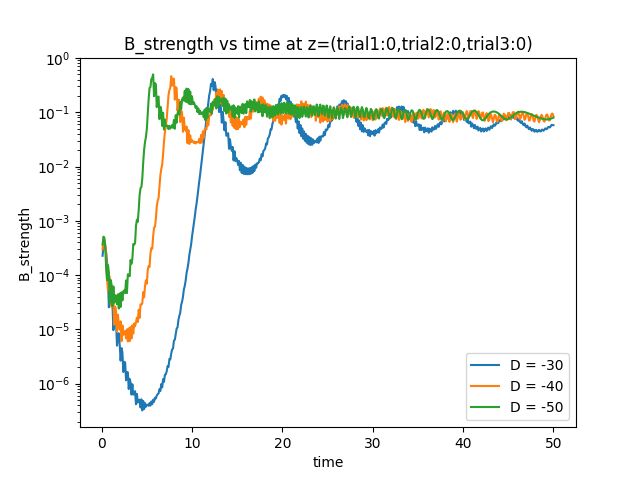
\includegraphics[width=\linewidth]{B_strength_vs_time_f_pos.png}
        \caption{Caption for the first figure}
        \label{fig:fig1}
    \end{minipage}
    \hfill
    \begin{minipage}{0.5\linewidth}
        \centering
        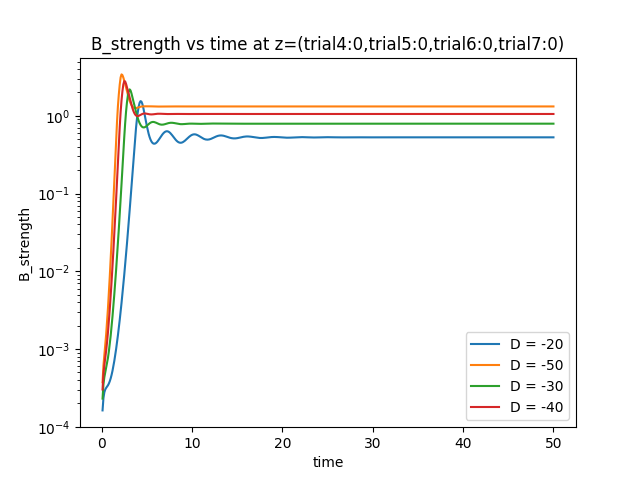
\includegraphics[width=\linewidth]{B_strength_vs_time.png}
        \caption{Caption for the second figure}
        \label{fig:fig2}
    \end{minipage}
\end{figure}
\section{The nvf.pdf draft}

In this new model, the direction chosen for the stratification relevant to the flux divergence is the same as in Sharanya's prior model in \texttt{nvf.pdf} (where \( \rho \) was stratified, not \( u \)), yet the direction of the flux divergence is now different. In \texttt{nvf.pdf}, we found oscillating near-equipartition solutions, similar to Sharanya's results for a particular flux sign. Given his findings, we anticipate that in this new model we will obtain steady near-equipartition solutions, as the flux divergence sign is reversed.
\begin{figure}[h]
    \centering
    \begin{minipage}{\linewidth}
        \centering
        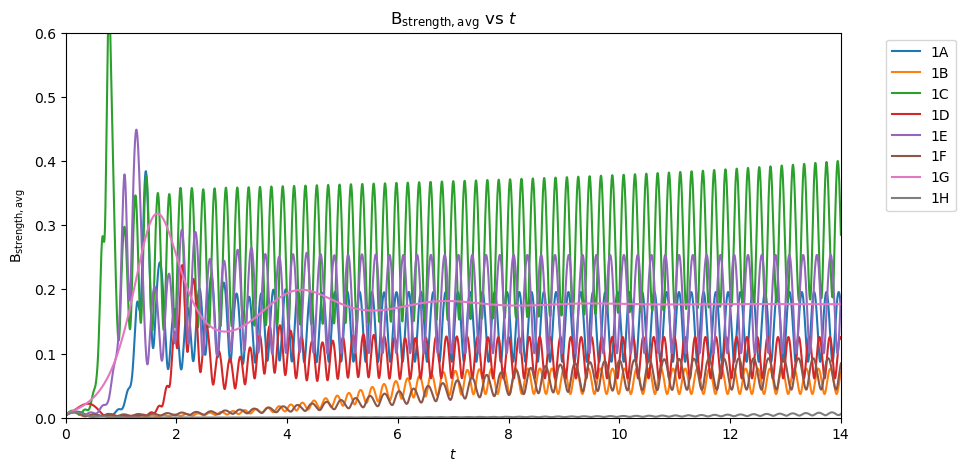
\includegraphics[width=\linewidth]{B_strength_avg_vs_time.png}
        \caption{(a) Caption for the first figure}
        \label{fig:fig1}
    \end{minipage}
    
    \vspace{0.5cm} % Adjust the space between figures as needed
    
    \begin{minipage}{\linewidth}
        \centering
        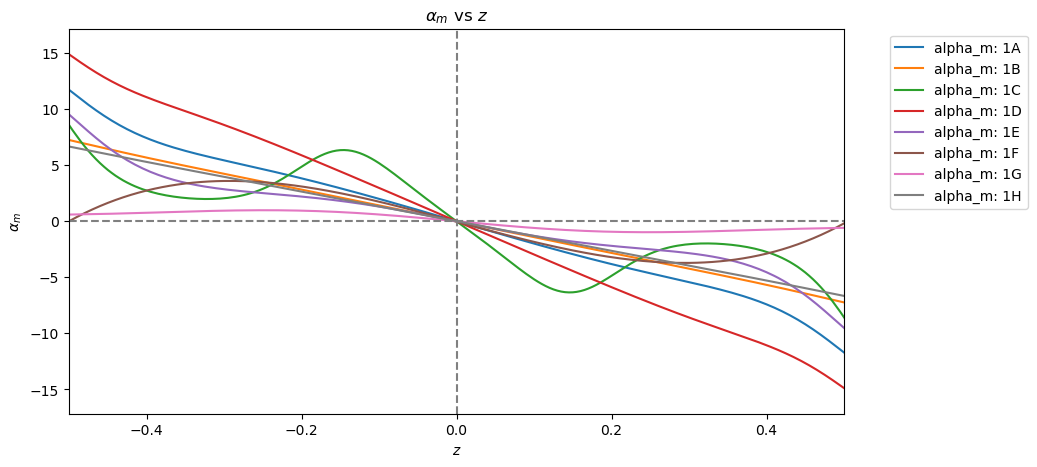
\includegraphics[width=\linewidth]{alpha_m_vs_z_final.png}
        \caption{(b) Caption for the second figure}
        \label{fig:fig2}
    \end{minipage}
\end{figure}

\section{2017 Notes}
\begin{figure}
    \centering
    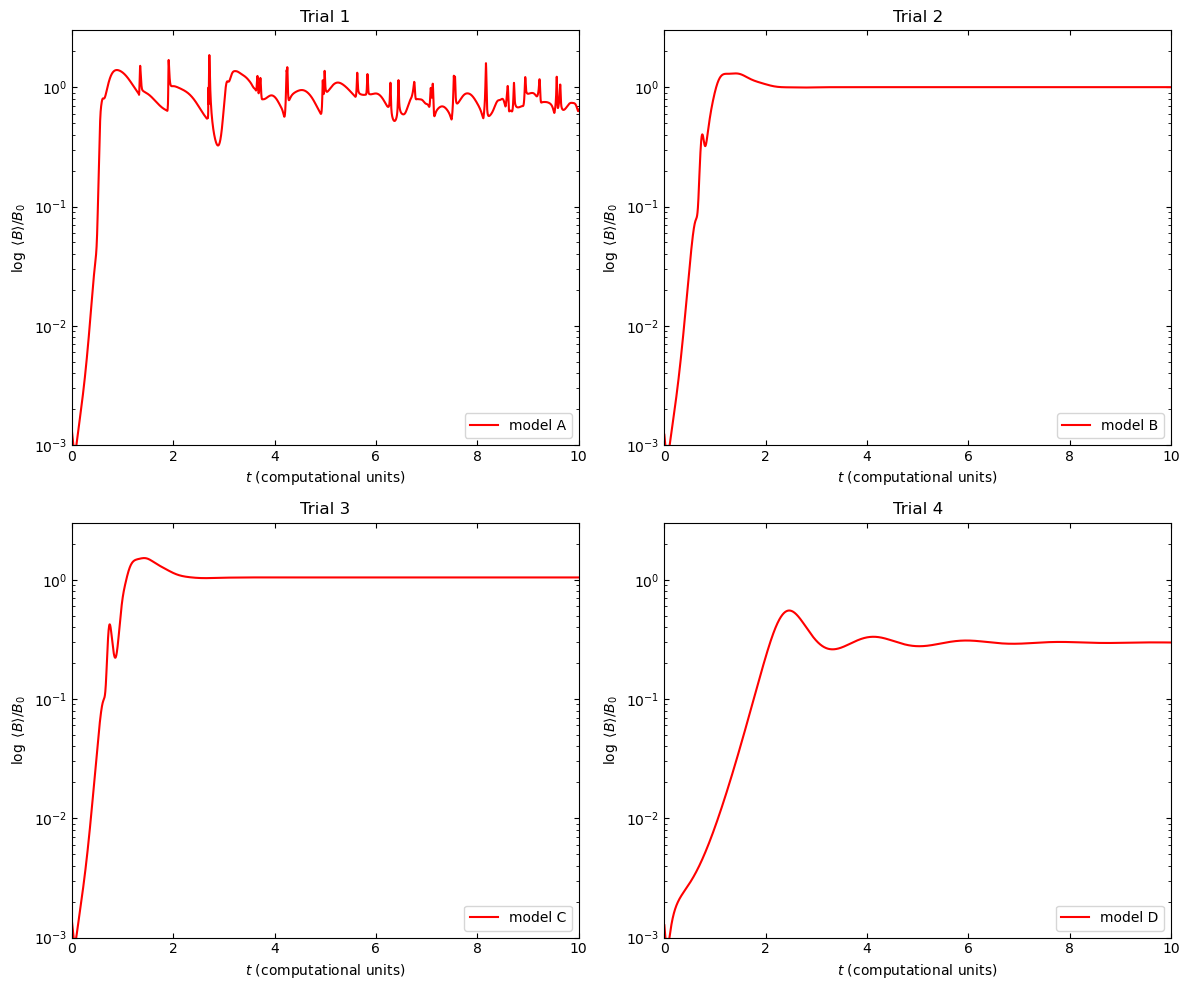
\includegraphics[width=\linewidth]{B_strength_avg_vs_time_subplots.png}
    \caption{Caption}
    \label{fig:enter-label}
\end{figure}

\begin{figure}
    \centering
    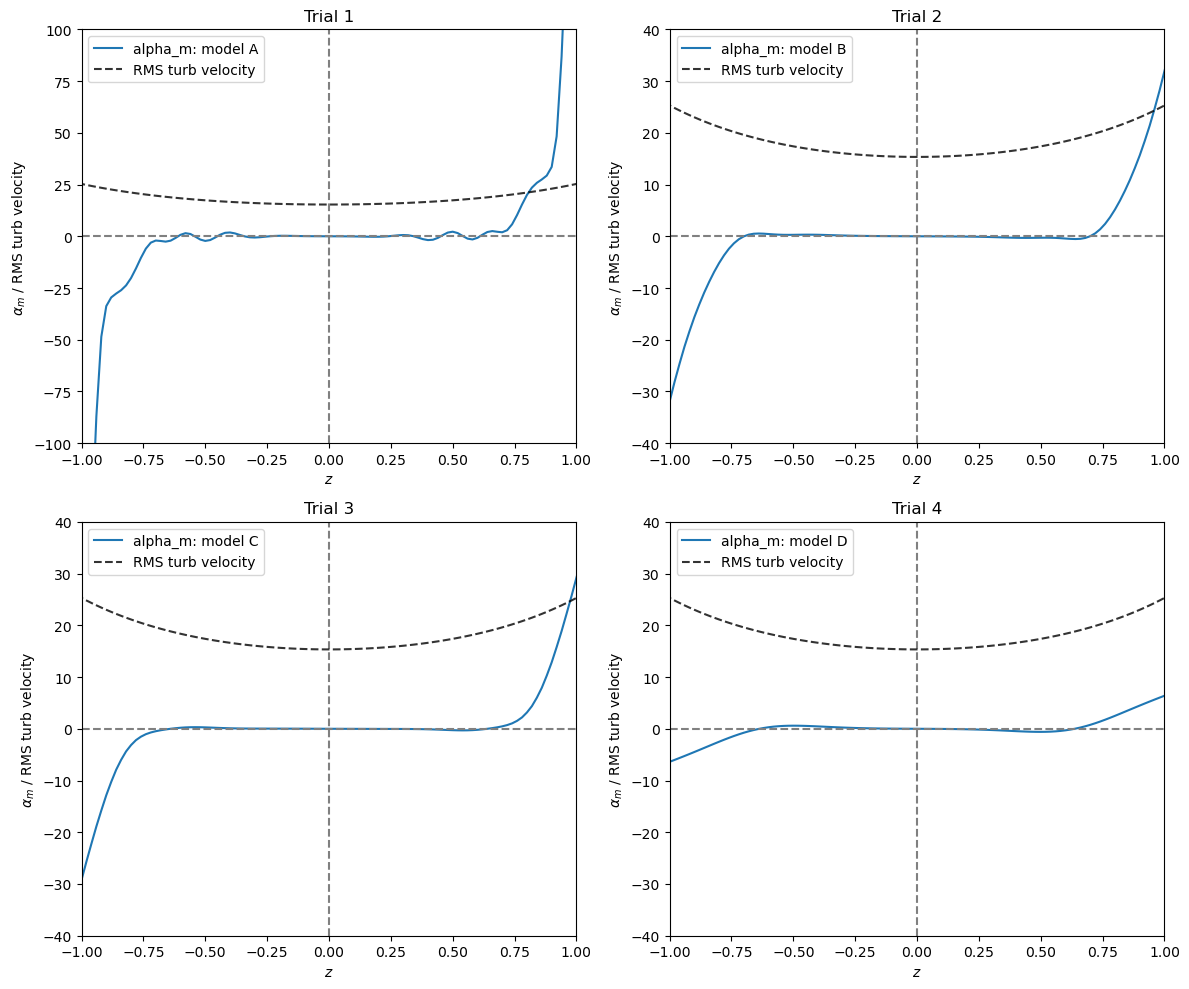
\includegraphics[width=\linewidth]{alpha_m_and_turb_vel_vs_z_subplots.png}
    \caption{Caption}
    \label{fig:enter-label}
\end{figure}


\begin{table}


\begin{center}
\caption{List of models for the new notes plots.}
\label{tab:models}
\begin{tabular}{lllllllll}
\hline
Model     &$R_\omega$   &$R_\alpha$   &$R_U$   &$R_\kappa$    &$f$      &$u$                          &$\rho$                     \\
\hline
%A= run 114
%B= run 115
%C= run 117
%D= run 119
A         &-20          &0            &0       &0             &1        &$\propto\exp[z^2/(2h^2)]$   &$\const$                   \\        
B         &-20          &0            &0.45    &0             &1        &$\propto\exp[z^2/(2h^2)]$   &$\const$                   \\  
C         &-20          &0            &0.45    &0             &1        &$\propto\exp[z^2/(2h^2)]$   &$\propto\exp[-z^2/h^2]$    \\ 
D         &-20          &0            &0.45    &0             &0.1      &$\propto\exp[z^2/(2h^2)]$   &$\const$                   \\  
\hline
\end{tabular}
\end{center}
\end{table}
%
\maketitle

%--------------------------------------------------------------------------------------------------------------------------------------------
\bibliographystyle{mn2e}
\bibliography{refs}

\label{lastpage}
\end{document}
